\chapter{As reações químicas: reagentes e produtos}\label{ch:g7:chemical-reactions}

O carvão brilha numa churrasqueira. Uma hora depois, quase nada sobrou
dos pedaços pretos --- um pouco de cinza cinzenta, e o calor que assou a
carne. Para onde foi o carbono preto? Ele não sumiu: ele encontrou o
oxigênio do \omterm{def:g4:air-a-mixture-of-gases:air}{ar} e virou um gás novo, invisível. Agora que conhecemos os
\omterm{def:g7:atoms-and-molecules:atom}{átomos} e as \omterm{def:g7:atoms-and-molecules:molecule}{moléculas}, podemos dizer exatamente o que acontece numa
transformação como essa.

\begin{recall}
Numa \omterm{def:g5:irreversible-changes:chemical-change}{transformação química} aparecem substâncias novas, e não há um
caminho simples de volta (\cref{ch:g5:irreversible-changes}). A água de
cal fica leitosa com o dióxido de carbono, o sulfato de cobre anidro
fica azul com a água (\cref{ch:g7:identifying-substances}). Toda a
matéria é feita de \omterm{def:g7:atoms-and-molecules:atom}{átomos}, que se agrupam em \omterm{def:g7:atoms-and-molecules:molecule}{moléculas}; uma fórmula como
\ce{CO2} lista os \omterm{def:g7:atoms-and-molecules:atom}{átomos} de uma \omterm{def:g7:atoms-and-molecules:molecule}{molécula}
(\cref{ch:g7:atoms-and-molecules}).
\end{recall}

\begin{omfigure}
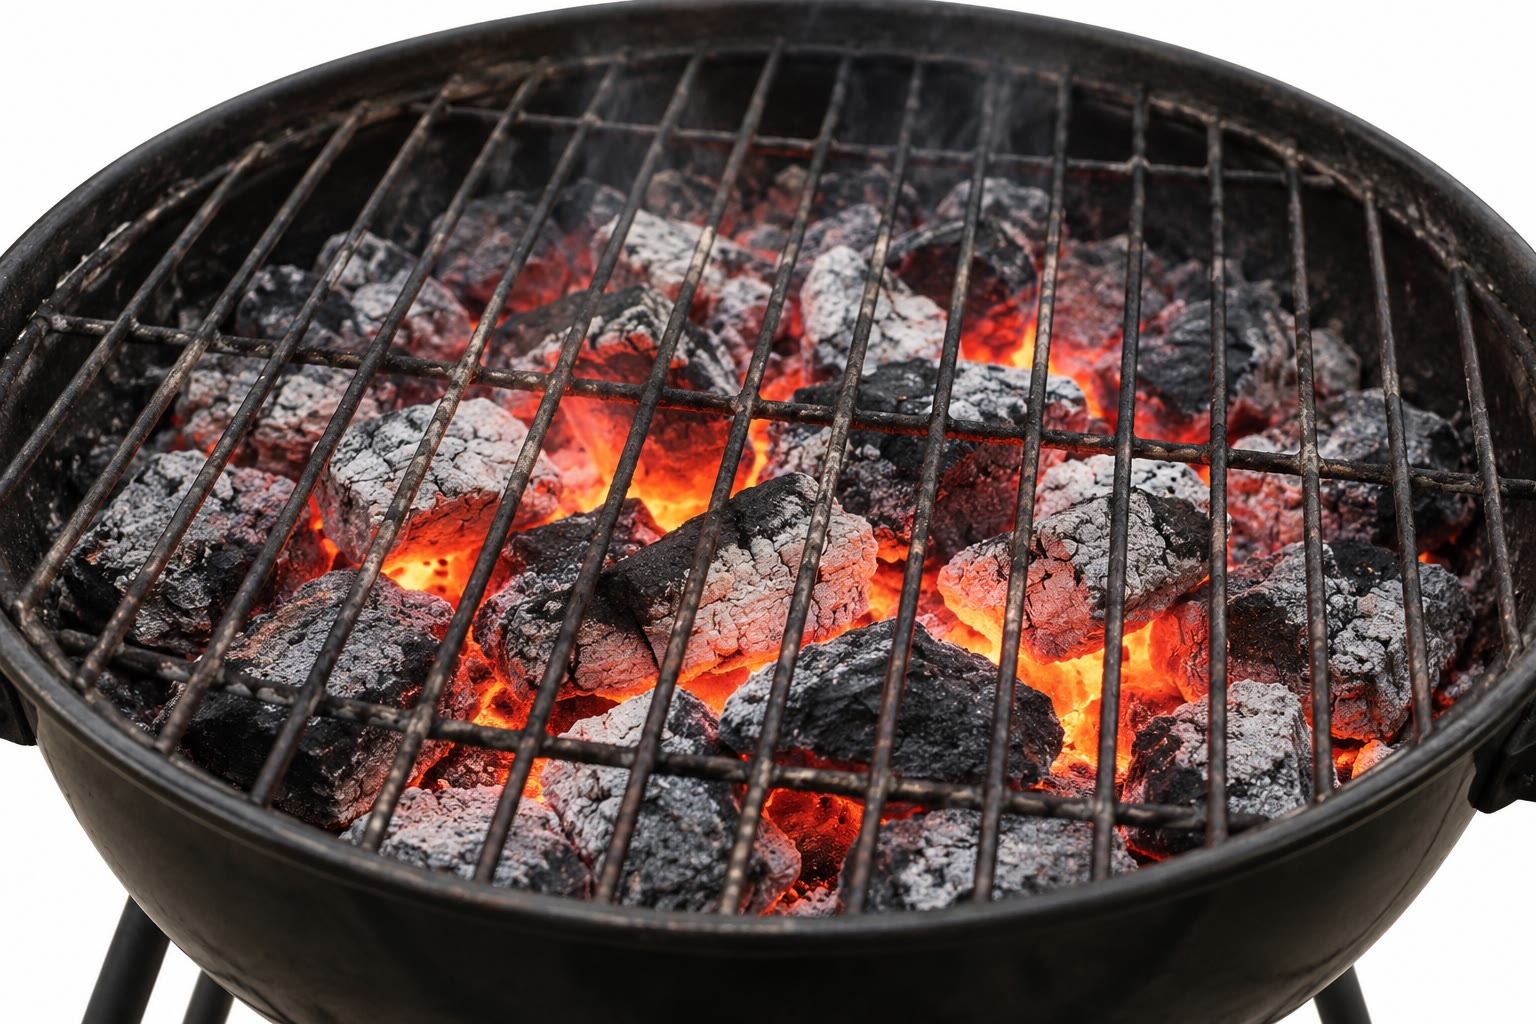
\includegraphics[width=0.55\linewidth]{images/book1/ai/g7-charcoal-bbq.jpg}

{\small Carvão em brasa: o carbono reagindo com o oxigênio do \omterm{def:g4:air-a-mixture-of-gases:air}{ar}.}
\end{omfigure}

\section{Transformações físicas e químicas}

\begin{definition}[Transformação física]\label{def:g7:chemical-reactions:physical-transformation}
Uma \emph{transformação física}\index{transformacao fisica@transformação física} muda o estado
ou a organização da matéria sem mudar as \omterm{def:g6:pure-substances-and-mixtures:species}{espécies químicas}: a fusão, a
solidificação, a ebulição, a dissolução, a \omterm{def:g6:pure-substances-and-mixtures:mixture}{mistura}. As mesmas espécies
estão presentes antes e depois; só a forma ou a organização delas mudou.
\end{definition}

\begin{example}[A água, de três jeitos]\label{ex:g7:chemical-reactions:water}
O gelo que derrete e vira água, a água que ferve e vira vapor de água, e
o sal que \omterm{def:g2:mixing-and-dissolving:dissolve}{se dissolve} na água são \omterm{def:g7:chemical-reactions:physical-transformation}{transformações físicas}: antes e
depois, há \omterm{def:g7:atoms-and-molecules:molecule}{moléculas} de água (e sal). Num zoom, as \omterm{def:g7:atoms-and-molecules:molecule}{moléculas} são as
mesmas; só mudou o modo como elas estão organizadas e como se movem.
\end{example}

\begin{proposition}[Transformação química]\label{prop:g7:chemical-reactions:chemical}
Numa \omterm{def:g5:irreversible-changes:chemical-change}{transformação química}, algumas \omterm{def:g6:pure-substances-and-mixtures:species}{espécies químicas} desaparecem e
aparecem espécies novas. Ela se distingue de uma \omterm{def:g7:chemical-reactions:physical-transformation}{transformação física}
pelos seus \omterm{def:g7:chemical-reactions:reactant}{produtos}: espécies novas, que podem ser detectadas com \omterm{def:g7:identifying-substances:characteristic-test}{testes
característicos}.
\end{proposition}
\begin{omfigure}
\begin{tikzpicture}[font=\small, level distance=1.5cm,
    box/.style={draw=omDef, fill=omDef!6, rounded corners=2pt, align=center,
      inner sep=4pt},
    level 1/.style={sibling distance=6.6cm},
    edge from parent/.style={draw, thick, omDef, ->}]
  \node[box] {uma transformação da matéria}
    child {node[box, text width=5.2cm] {\textbf{física}: as mesmas espécies\\
      antes e depois\\ \footnotesize fusão, ebulição, dissolução, mistura}}
    child {node[box, draw=omProp, fill=omProp!6, text width=5.2cm]
      {\textbf{química}: espécies desaparecem,\\ espécies novas aparecem\\
      \footnotesize combustão, ferrugem, cozimento}};
\end{tikzpicture}

{\small Dois tipos de transformação.}
\end{omfigure}

\section{Reagentes e produtos}

\begin{definition}[Reação química]\label{def:g7:chemical-reactions:reaction}
Uma \emph{reação química}\index{reacao quimica@reação química} é o modelo que os
químicos usam para uma \omterm{def:g5:irreversible-changes:chemical-change}{transformação química}: ela lista as espécies que
são consumidas e as espécies que são formadas.
\end{definition}

\begin{definition}[Reagentes e produtos]\label{def:g7:chemical-reactions:reactant}
As espécies consumidas numa \omterm{def:g7:chemical-reactions:reaction}{reação química} são os
\emph{reagentes}\index{reagente}; as espécies formadas são os
\emph{produtos}\index{produto}.
\end{definition}

\begin{example}[O carbono queimando no oxigênio]\label{ex:g7:chemical-reactions:carbon}
Quando o carvão \omterm{def:g4:what-a-fire-needs:burning}{queima}, os \omterm{def:g7:chemical-reactions:reactant}{reagentes} são o carbono (o carvão) e o
oxigênio (do \omterm{def:g4:air-a-mixture-of-gases:air}{ar}). O \omterm{def:g7:chemical-reactions:reactant}{produto} é o dióxido de carbono: sacudido com água de
cal, o gás que fica no frasco a deixa leitosa.
\end{example}

\begin{inthelab}[Carvão num frasco de oxigênio]
O professor aquece um pedacinho de carvão até ele ficar em brasa, numa
colher de \omterm{def:g4:what-a-fire-needs:burning}{combustão}, e depois o desce para dentro de um frasco de
oxigênio. O carvão brilha muito mais do que no \omterm{def:g4:air-a-mixture-of-gases:air}{ar} e vai encolhendo até
sumir. O frasco é tampado, um pouco de água de cal é despejado nele e
sacudido: ela fica leitosa. O carbono e o oxigênio foram consumidos; foi
formado dióxido de carbono.
\end{inthelab}

\begin{omfigure}
\begin{tikzpicture}[font=\small, scale=1.3]
  \pic[transform shape] at (0,0) {gasjaropen={0}{white}};
  \fill[omWater!60] (-0.68,2.62) rectangle (0.68,2.7);
  \draw[omGlass, line width=0.4pt] (-0.68,2.62) rectangle (0.68,2.7);
  \draw[black!60, line width=1.2pt] (0.15,2.7) -- (0.15,3.6) -- (1.2,3.6);
  \draw[black!60, line width=1.2pt] (0.15,2.7) -- (0.15,1.2);
  \fill[black!60] (-0.12,1.12) rectangle (0.32,1.2);
  \fill[red!70!black] (0.0,1.32) circle (0.13);
  \fill[orange!90!yellow] (0.0,1.32) circle (0.08);
  \draw[<-, omProp, thick] (0.15,1.35) -- (1.5,1.6) node[right, text=black]
    {carvão em brasa (carbono)};
  \draw[<-, omProp, thick] (-0.35,2.1) -- (1.5,2.3) node[right, text=black]
    {oxigênio};
  \draw[<-, omProp, thick] (0.6,2.66) -- (1.5,2.95) node[right, text=black]
    {tampa};
  \draw[<-, omProp, thick] (0.15,3.1) -- (1.5,3.6) node[right, text=black]
    {colher de combustão};
\end{tikzpicture}

{\small Carvão em brasa, descido numa colher para dentro de um frasco de
oxigênio, \omterm{def:g4:what-a-fire-needs:burning}{queima} com um brilho forte: o carbono e o oxigênio reagem e
formam dióxido de carbono.}
\end{omfigure}

\begin{example}[A palha de aço]\label{ex:g7:chemical-reactions:steel-wool}
Um chumaço de palha de aço fina, que é principalmente ferro, pode
queimar no \omterm{def:g4:air-a-mixture-of-gases:air}{ar} soltando chuvas de faíscas. Os \omterm{def:g7:chemical-reactions:reactant}{reagentes} são o ferro e o
oxigênio; o \omterm{def:g7:chemical-reactions:reactant}{produto} é um sólido escuro e quebradiço, um óxido de ferro.
\end{example}

\begin{omfigure}
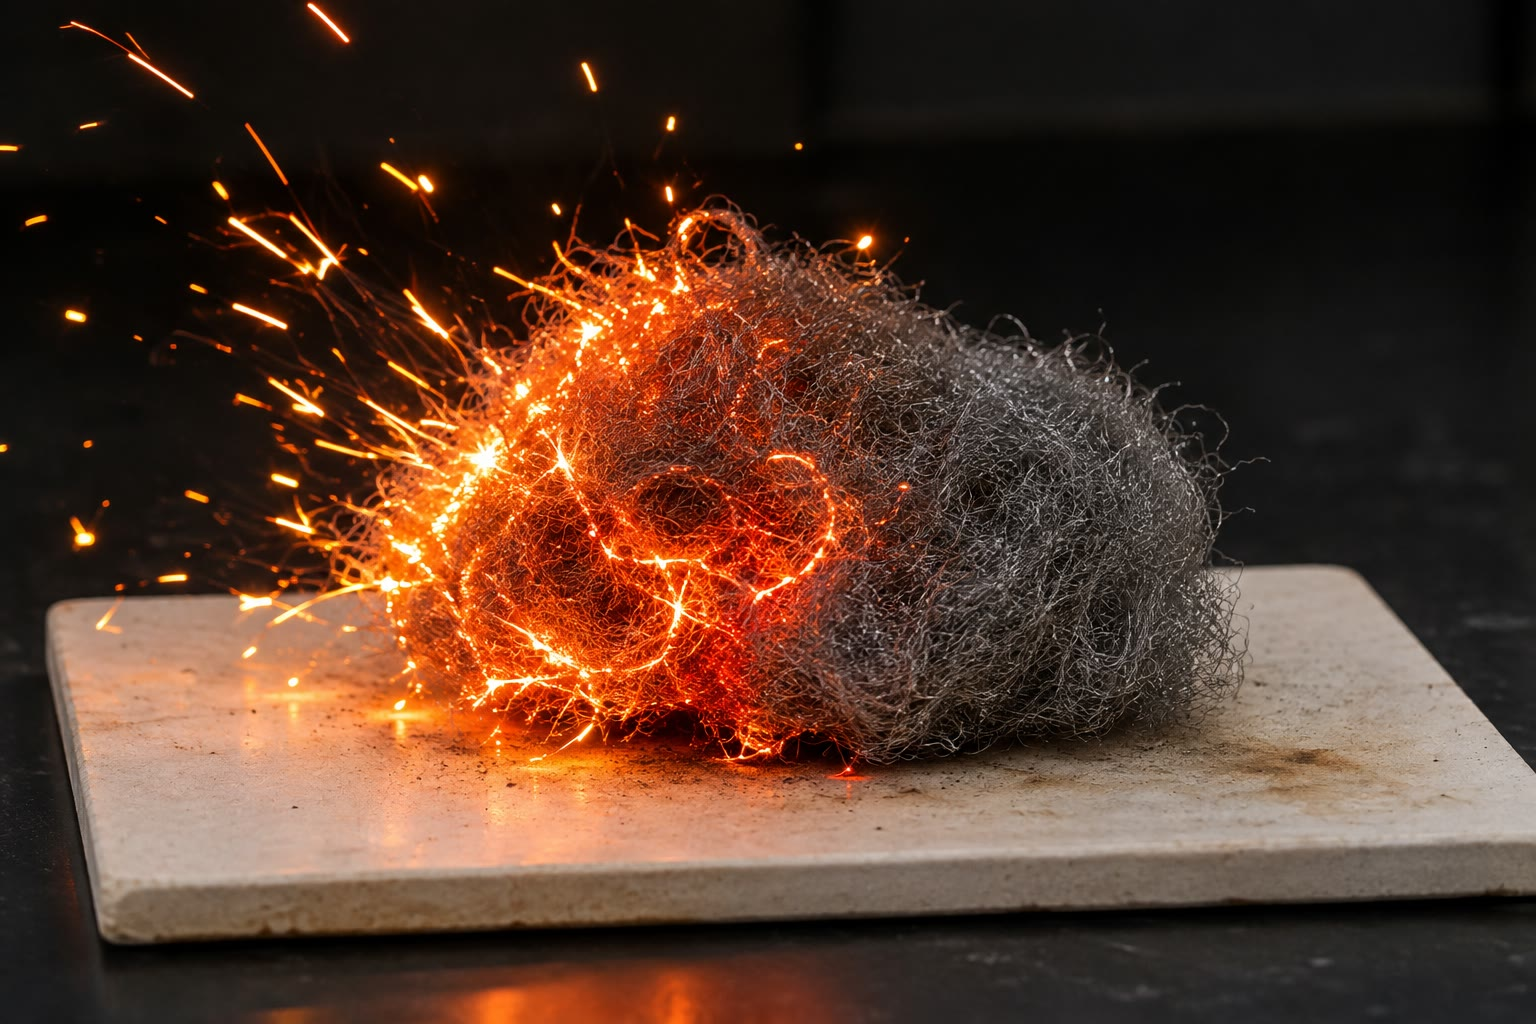
\includegraphics[width=0.5\linewidth]{images/book1/ai/g7-steel-wool-burning.jpg}

{\small Palha de aço queimando no laboratório: o ferro e o oxigênio
reagem.}
\end{omfigure}

\section{A equação por extenso}

\begin{definition}[Equação por extenso]\label{def:g7:chemical-reactions:word-equation}
Uma \emph{equação por extenso}\index{equacao por extenso@equação por extenso} escreve uma
\omterm{def:g7:chemical-reactions:reaction}{reação química} em palavras: os nomes dos \omterm{def:g7:chemical-reactions:reactant}{reagentes} à esquerda, ligados
por $+$, uma seta, e os nomes dos \omterm{def:g7:chemical-reactions:reactant}{produtos} à direita. A seta se lê
``reagem e dão''.
\end{definition}

\begin{example}[Três equações por extenso]\label{ex:g7:chemical-reactions:three}
\begin{center}
\begin{tabular}{l}
carbono $+$ oxigênio $\longrightarrow$ dióxido de carbono\\[2pt]
metano $+$ oxigênio $\longrightarrow$ dióxido de carbono $+$ água\\[2pt]
ferro $+$ oxigênio $\longrightarrow$ óxido de ferro
\end{tabular}
\end{center}
\end{example}

\begin{method}[Escrever uma equação por extenso]\label{met:g7:chemical-reactions:write}
\begin{enumerate}
  \item Encontre os \omterm{def:g7:chemical-reactions:reactant}{reagentes}: as espécies que desaparecem.
  \item Encontre os \omterm{def:g7:chemical-reactions:reactant}{produtos}: as espécies novas, identificadas por
        testes.
  \item Escreva os \omterm{def:g7:chemical-reactions:reactant}{reagentes} à esquerda, os \omterm{def:g7:chemical-reactions:reactant}{produtos} à direita, com uma
        seta entre eles; nunca um sinal de igual.
\end{enumerate}
Uma espécie que está presente mas não participa --- o nitrogênio do \omterm{def:g4:air-a-mixture-of-gases:air}{ar}
em volta de uma chama --- não é escrita.
\end{method}

\section{Uma reação é um rearranjo de átomos}

\begin{proposition}[Os átomos são rearranjados]\label{prop:g7:chemical-reactions:rearranged}
Numa \omterm{def:g7:chemical-reactions:reaction}{reação química}, as \omterm{def:g7:atoms-and-molecules:molecule}{moléculas} dos \omterm{def:g7:chemical-reactions:reactant}{reagentes} se desfazem e os \omterm{def:g7:atoms-and-molecules:atom}{átomos}
delas se juntam de outro modo para construir as \omterm{def:g7:atoms-and-molecules:molecule}{moléculas} dos \omterm{def:g7:chemical-reactions:reactant}{produtos}.
Os próprios \omterm{def:g7:atoms-and-molecules:atom}{átomos} não são criados nem destruídos: os mesmos \omterm{def:g7:atoms-and-molecules:atom}{átomos}, nos
mesmos números, estão lá antes e depois.
\end{proposition}

\begin{example}[O metano queimando, molécula por molécula]\label{ex:g7:chemical-reactions:methane}
Quando o metano de um fogão a gás \omterm{def:g4:what-a-fire-needs:burning}{queima}, uma \omterm{def:g7:atoms-and-molecules:molecule}{molécula} de metano
\ce{CH4} encontra duas \omterm{def:g7:atoms-and-molecules:molecule}{moléculas} de oxigênio \ce{O2}. Os \omterm{def:g7:atoms-and-molecules:atom}{átomos} delas se
rearranjam numa \omterm{def:g7:atoms-and-molecules:molecule}{molécula} de dióxido de carbono \ce{CO2} e duas \omterm{def:g7:atoms-and-molecules:molecule}{moléculas}
de água \ce{H2O}. Antes: 1 \omterm{def:g7:atoms-and-molecules:atom}{átomo} de carbono, 4 de hidrogênio e 4 de
oxigênio. Depois: 1 de carbono, 4 de hidrogênio e $2 + 2 = 4$ de
oxigênio. Nada se perde, nada aparece do nada.
\end{example}

\begin{omfigure}
\begin{tikzpicture}[font=\small]
  % methane
  \begin{scope}[xshift=0cm]
    \node[aC] (c) at (0,0) {};
    \node[aH] (h1) at (0,0.78) {}; \node[aH] (h2) at (-0.74,-0.3) {};
    \node[aH] (h3) at (0.74,-0.3) {}; \node[aH] (h4) at (0.2,-0.68) {};
    \begin{scope}[on background layer]
      \foreach \h in {h1,h2,h3,h4} \draw[bond] (c.center) -- (\h.center);
    \end{scope}
    \node at (0,-1.2) {1 metano};
  \end{scope}
  \node at (1.45,0) {$+$};
  % two oxygen molecules
  \foreach \y in {0.45,-0.45} {
    \node[aO] (a) at (2.4,\y) {}; \node[aO] (b) at (3.05,\y) {};
    \begin{scope}[on background layer]
      \draw[bond, line width=1.1pt] ([yshift=1.6pt]a.center) -- ([yshift=1.6pt]b.center);
      \draw[bond, line width=1.1pt] ([yshift=-1.6pt]a.center) -- ([yshift=-1.6pt]b.center);
    \end{scope}
  }
  \node at (2.72,-1.2) {2 oxigênio};
  \draw[->, thick, omProp] (3.8,0) -- (5.0,0);
  % carbon dioxide
  \begin{scope}[xshift=6.3cm]
    \node[aO] (a) at (-0.8,0) {}; \node[aC] (c) at (0,0) {}; \node[aO] (b) at (0.8,0) {};
    \begin{scope}[on background layer]
      \foreach \d in {-1.6,1.6} {
        \draw[bond, line width=1.1pt] ([yshift=\d pt]a.center) -- ([yshift=\d pt]c.center);
        \draw[bond, line width=1.1pt] ([yshift=\d pt]c.center) -- ([yshift=\d pt]b.center);}
    \end{scope}
    \node at (0,-1.2) {1 dióxido de carbono};
  \end{scope}
  \node at (7.8,0) {$+$};
  % two water molecules
  \foreach \x in {8.9,10.6} {
    \node[aO] (o) at (\x,0.2) {};
    \node[aH] (p) at (\x-0.58,-0.25) {}; \node[aH] (q) at (\x+0.58,-0.25) {};
    \begin{scope}[on background layer]
      \draw[bond] (o.center) -- (p.center); \draw[bond] (o.center) -- (q.center);
    \end{scope}
  }
  \node at (9.75,-1.2) {2 água};
  % atom counts
  \node[align=center, font=\footnotesize] at (1.5,-2.0) {antes: 1 C, 4 H, 4 O};
  \node[align=center, font=\footnotesize] at (8.5,-2.0) {depois: 1 C, 4 H, 4 O};
\end{tikzpicture}

{\small O metano queimando, desenhado com modelos moleculares: os \omterm{def:g7:atoms-and-molecules:atom}{átomos}
dos \omterm{def:g7:chemical-reactions:reactant}{reagentes} se rearranjam nos \omterm{def:g7:chemical-reactions:reactant}{produtos}. Os mesmos \omterm{def:g7:atoms-and-molecules:atom}{átomos} são contados
antes e depois.}
\end{omfigure}

\begin{remark}[Contar as moléculas]\label{rem:g7:chemical-reactions:counting}
A \omterm{def:g7:chemical-reactions:word-equation}{equação por extenso} não diz quantas \omterm{def:g7:atoms-and-molecules:molecule}{moléculas} reagem: para isso, a
equação é escrita com fórmulas e com números na frente delas. Escrever
essas equações, e encontrar os números certos, é o assunto de um
capítulo mais adiante.
\end{remark}

\section{Exercícios}

\begin{exercise}[$\star$]\label{exo:g7:chemical-reactions:1}
\omterm{def:g7:chemical-reactions:physical-transformation}{Transformação física} ou química? O gelo derretendo, um fósforo
queimando, o açúcar se dissolvendo, o pão torrando, um prego
enferrujando.
\end{exercise}

\begin{exercise}[$\star$]\label{exo:g7:chemical-reactions:2}
O que são os \omterm{def:g7:chemical-reactions:reactant}{reagentes} e os \omterm{def:g7:chemical-reactions:reactant}{produtos} de uma \omterm{def:g7:chemical-reactions:reaction}{reação química}?
\end{exercise}

\begin{exercise}[$\star$]\label{exo:g7:chemical-reactions:3}
Escreva a \omterm{def:g7:chemical-reactions:word-equation}{equação por extenso} da \omterm{def:g4:what-a-fire-needs:burning}{queima} do carbono no oxigênio.
\end{exercise}

\begin{exercise}[$\star$]\label{exo:g7:chemical-reactions:4}
Na \omterm{def:g7:chemical-reactions:word-equation}{equação por extenso} ``ferro $+$ oxigênio $\longrightarrow$ óxido de
ferro'', diga quais são os \omterm{def:g7:chemical-reactions:reactant}{reagentes} e qual é o \omterm{def:g7:chemical-reactions:reactant}{produto}.
\end{exercise}

\begin{exercise}[$\star\star$]\label{exo:g7:chemical-reactions:5}
Quando o metano \omterm{def:g4:what-a-fire-needs:burning}{queima}, um copo frio segurado acima da chama fica
embaçado, e o gás recolhido turva a água de cal. Que \omterm{def:g7:chemical-reactions:reactant}{produtos} esses dois
testes mostram?
\end{exercise}

\begin{exercise}[$\star\star$]\label{exo:g7:chemical-reactions:6}
O zinco reage com o ácido clorídrico: o zinco desaparece, bolhas de
hidrogênio são liberadas, e o cloreto de zinco fica na solução. Escreva
a \omterm{def:g7:chemical-reactions:word-equation}{equação por extenso}.
\end{exercise}

\begin{exercise}[$\star\star$]\label{exo:g7:chemical-reactions:7}
Olhe a figura com os modelos do metano queimando. Conte os \omterm{def:g7:atoms-and-molecules:atom}{átomos} de
hidrogênio antes e depois da reação.
\end{exercise}

\begin{exercise}[$\star\star$]\label{exo:g7:chemical-reactions:8}
Por que \omterm{def:g2:mixing-and-dissolving:dissolve}{dissolver} sal na água não é uma \omterm{def:g7:chemical-reactions:reaction}{reação química}, embora o sal
suma da vista?
\end{exercise}

\begin{exercise}[$\star\star$]\label{exo:g7:chemical-reactions:9}
Uma tora de madeira \omterm{def:g4:what-a-fire-needs:burning}{queima} até virar um montinho de cinza. Explique,
usando a palavra ``\omterm{def:g7:chemical-reactions:reactant}{produtos}'', por que a cinza é tão mais leve do que a
tora.
\end{exercise}

\begin{exercise}[$\star\star$]\label{exo:g7:chemical-reactions:10}
O hidrogênio \omterm{def:g4:what-a-fire-needs:burning}{queima} no oxigênio e dá apenas água. Escreva a \omterm{def:g7:chemical-reactions:word-equation}{equação por
extenso}, e diga que teste identificaria o \omterm{def:g7:chemical-reactions:reactant}{produto}.
\end{exercise}

\begin{exercise}[$\star\star\star$]\label{exo:g7:chemical-reactions:11}
Duas \omterm{def:g7:atoms-and-molecules:molecule}{moléculas} de hidrogênio \ce{H2} reagem com uma \omterm{def:g7:atoms-and-molecules:molecule}{molécula} de oxigênio
\ce{O2} e dão duas \omterm{def:g7:atoms-and-molecules:molecule}{moléculas} de água \ce{H2O}. Conte os \omterm{def:g7:atoms-and-molecules:atom}{átomos} de cada
tipo antes e depois, e mostre que nenhum foi criado ou destruído.
\end{exercise}

\begin{exercise}[$\star\star\star$]\label{exo:g7:chemical-reactions:12}
Um aluno desenha a \omterm{def:g4:what-a-fire-needs:burning}{queima} do carbono assim: um \omterm{def:g7:atoms-and-molecules:atom}{átomo} de carbono $+$ uma
\omterm{def:g7:atoms-and-molecules:molecule}{molécula} de oxigênio $\longrightarrow$ uma \omterm{def:g7:atoms-and-molecules:molecule}{molécula} de dióxido de
carbono e um \omterm{def:g7:atoms-and-molecules:atom}{átomo} de oxigênio que sobra. O que está errado nesse
desenho? Descreva em palavras o desenho correto.
\end{exercise}

\section{Problema: dentro da chama de um fogão a gás}

\begin{problem}[{Problema de fim de semana --- o que queima na chama de
um fogão a gás, o que ela produz e quantas moléculas participam}]
\label{pb:g7:chemical-reactions:1}
O gás de um fogão de cozinha é principalmente metano, \ce{CH4}. Na chama
azul, o metano reage com o oxigênio do \omterm{def:g4:air-a-mixture-of-gases:air}{ar}. Num laboratório, o professor
segura por alguns segundos um béquer frio e seco, de boca para baixo,
acima de uma chama assim; depois desvira o béquer, despeja nele um pouco
de água de cal e o sacode.

\medskip
\noindent\textbf{Parte I --- \omterm{def:g7:chemical-reactions:reactant}{Reagentes} e \omterm{def:g7:chemical-reactions:reactant}{produtos}.}
\begin{enumerate}
  \item Dê o nome dos dois \omterm{def:g7:chemical-reactions:reactant}{reagentes} dessa reação.
  \item Aparecem gotinhas dentro do béquer frio; uma delas deixa azul o
        sulfato de cobre anidro. Que \omterm{def:g7:chemical-reactions:reactant}{produto} isso mostra?
  \item A água de cal fica leitosa. Que outro \omterm{def:g7:chemical-reactions:reactant}{produto} isso mostra?
  \item O \omterm{def:g4:air-a-mixture-of-gases:air}{ar} também contém nitrogênio, que atravessa a chama sem mudar.
        O nitrogênio é um \omterm{def:g7:chemical-reactions:reactant}{reagente}? Ele deve aparecer na \omterm{def:g7:chemical-reactions:word-equation}{equação por
        extenso}?
\end{enumerate}

\medskip
\noindent\textbf{Parte II --- A \omterm{def:g7:chemical-reactions:word-equation}{equação por extenso}.}
\begin{enumerate}[resume]
  \item Escreva a \omterm{def:g7:chemical-reactions:word-equation}{equação por extenso} da reação.
  \item A \omterm{def:g4:what-a-fire-needs:burning}{queima} do metano é uma \omterm{def:g7:chemical-reactions:physical-transformation}{transformação física} ou química? Dê
        duas razões.
  \item Escreva as fórmulas das quatro espécies da reação.
\end{enumerate}

\medskip
\noindent\textbf{Parte III --- Contar as \omterm{def:g7:atoms-and-molecules:molecule}{moléculas}.}
Cada \omterm{def:g7:atoms-and-molecules:molecule}{molécula} de metano que \omterm{def:g4:what-a-fire-needs:burning}{queima} reage com duas \omterm{def:g7:atoms-and-molecules:molecule}{moléculas} de oxigênio
e dá uma \omterm{def:g7:atoms-and-molecules:molecule}{molécula} de dióxido de carbono e duas \omterm{def:g7:atoms-and-molecules:molecule}{moléculas} de água.
\begin{enumerate}[resume]
  \item Conte os \omterm{def:g7:atoms-and-molecules:atom}{átomos} de carbono, de hidrogênio e de oxigênio numa
        \omterm{def:g7:atoms-and-molecules:molecule}{molécula} de metano e em duas \omterm{def:g7:atoms-and-molecules:molecule}{moléculas} de oxigênio, juntas.
  \item Conte-os numa \omterm{def:g7:atoms-and-molecules:molecule}{molécula} de dióxido de carbono e em duas \omterm{def:g7:atoms-and-molecules:molecule}{moléculas}
        de água, juntas. O que você observa?
  \item A chama \omterm{def:g4:what-a-fire-needs:burning}{queima} 10 \omterm{def:g7:atoms-and-molecules:molecule}{moléculas} de metano. Quantas \omterm{def:g7:atoms-and-molecules:molecule}{moléculas} de
        oxigênio ela consome?
  \item Quantas \omterm{def:g7:atoms-and-molecules:molecule}{moléculas} de dióxido de carbono ela produz?
  \item Quantas \omterm{def:g7:atoms-and-molecules:molecule}{moléculas} de água ela produz?
\end{enumerate}
\end{problem}
